\documentclass{article}
\usepackage[utf8]{inputenc}
\usepackage{amsmath, amssymb, amsfonts, amsthm}
\usepackage{enumitem}
\usepackage{mathrsfs}
\usepackage[colorlinks=true]{hyperref}
\usepackage{mathtools}
\usepackage{xypic}
\usepackage{centernot}
\usepackage{biblatex}
\usepackage[capitalize, nameinlink]{cleveref}
\newtheorem{theorem}{Theorem}[section]
\newtheorem{exercise}{Exercise}[section]
\newtheorem{prop}{Proposition}
\newtheorem{definition}{Definition}
\newtheorem{corollary}{Corollary}[theorem]
\newtheorem{lemma}[theorem]{Lemma}
\bibliography{References}

\newcommand{\Vars}{\mathrm{Vars}}
\newcommand{\justif}[2]{&{#1}&\text{#2}}

\DeclareUnicodeCharacter{2212}{-}


\title{CS228 Tutorial Solutions}
\author{Arpon Basu}

\begin{document}
\maketitle
\tableofcontents
\pagebreak
\section{Tutorial 1}
\subsection*{Exercise 2.6}
Let $p_T$ be the propositional variable denoting if $T$ is good, where $T\in\{A, B, C\}$. 
Then the puzzle can be encoded as 
$$(p_A\Leftrightarrow (\lnot p_A\wedge\lnot p_B\wedge\lnot p_C))$$
$$\bigwedge (p_B\Leftrightarrow ((p_A\wedge\lnot p_B\wedge\lnot p_C)\lor (\lnot p_A\wedge p_B\wedge\lnot p_C)\lor (\lnot p_A\wedge\lnot p_B\wedge p_C)))$$
\subsection*{Exercise 2.7}
Consider the ``let''-expression 
$$\mathrm{let}\; p_0 = (\mathrm{let}\; p_1 = (\mathrm{let}\; p_2 = (\ldots) \;\mathrm{in}\; p_2\wedge p_2) \;\mathrm{in}\; p_1\wedge p_1) \;\mathrm{in}\; p_0\wedge p_0$$
This expression, in linear length, represents a formula of exponential size.
\subsection*{Exercise 3.10}
We will not write $m(\cdot)$ in the top row for brevity.
\begin{enumerate}[label=(\alph*)]
    \item \[
        \begin{array}{|c|c|c|c|c|}
            \hline
        p & q & p\to q & \lnot p & \lnot p\lor q \\
        \hline
        1 & 1 & 1 & 0 & 1 \\
        1 & 0 & 0 & 0 & 0 \\
        0 & 1 & 1 & 1 & 1 \\
        0 & 0 & 1 & 1 & 1 \\
        \hline
        \end{array}
        \]
    \item DIY
    \item  \[
    \begin{array}{|c|c|c|c|c|c|c|c|}
        \hline
    p & q & p\oplus q & \lnot p & \lnot q & \lnot p\wedge q & p\wedge\lnot q & (\lnot p\wedge q)\lor(p\wedge \lnot q)\\
    \hline
    1 & 1 & 0 & 0 & 0 & 0 & 0 & 0\\
    1 & 0 & 1 & 0 & 1 & 0 & 1 & 1\\
    0 & 1 & 1 & 1 & 0 & 1 & 0 & 1\\
    0 & 0 & 0 & 1 & 1 & 0 & 0 & 0\\
    \hline
    \end{array}
    \]
    \item DIY
\end{enumerate}
\subsection*{Exercise 3.23}
Consider the model $m$, where $m[p] = 1$ if and only if $p\in\Sigma$. \\
Assume for the sake of contradiction that $m\not\models\Sigma$, and thus let $H$ be \emph{a smallest} \footnote{note that every formula in propositional logic can be generated in finitely many steps from the base cases. Consequently, for every formula $F$, there is a minimum number of steps `$k$' needed to generate $F$, and we call $k$ the \emph{size} of $F$. Once we have defined a finite size for every formula, we can talk about \emph{a} smallest formula of some subset of formulae} formula such that $m\not\models H$. Note that if the root connective of $H$ is $\lnot$, then $H$ has at least 2 connectives in it by the properties of $m$ \footnote{If $H$ is of the form $\lnot F$ and $F$ doesn't have any further connectives, then $H$ is $\lnot p$ for some propositional variable $p$ and $m$ satisfies it by definition}, and then by the rules of generating formulae, $H$ must be of the form $\lnot\lnot F, F\wedge G, F\lor G, \lnot(F\lor G)$ or $\lnot(F\wedge G)$ for some formulae $F, G$. Now, 
\begin{enumerate}
    \item $H = \lnot\lnot F$: Since $H\in\Sigma$, $F\in\Sigma$. But since $m\not\models H$, $m\not\models F$. But $F$ is a strictly smaller formula than $H$. Thus this case is not possible.
    \item $H = F\wedge G$: Since $H\in\Sigma$, $F, G\in\Sigma$. But since $m\not\models H$, either $m\not\models F$ or $m\not\models G$. But $F, G$ are strictly smaller than $H$. Thus this case is not possible.
    \item $H = F\lor G$: Since $H\in\Sigma$, either $F\in\Sigma$ or $G\in\Sigma$. But since $m\not\models H$, $m\not\models F$ and $m\not\models G$. But $F, G$ are strictly smaller than $H$. Thus this case is not possible.
    \item $H = \lnot(F\lor G)$: Since $H\in\Sigma$, $\lnot F, \lnot G\in\Sigma$. But since $m\not\models H$, $m\models (F\lor G)$, and thus $m\models F$ or $m\models G$, implying $m\not\models \lnot F$ or $m\not\models \lnot G$. But $\lnot F, \lnot G$ are strictly smaller than $H$. Thus this case is not possible.
    \item $H = \lnot(F\wedge G)$: Since $H\in\Sigma$, either $\lnot F\in\Sigma$ or $\lnot G\in\Sigma$. But since $m\not\models H$, $m\models (F\wedge G)$, and thus $m\models F$ and $m\models G$, implying $m\not\models \lnot F$ and $m\not\models \lnot G$. But $\lnot F, \lnot G$ are strictly smaller than $H$. Thus this case is not possible.
\end{enumerate}
Consequently, we arrive at a contradiction. Thus $m\models\Sigma$, ie:- $\Sigma$ is satisfiable.
\subsection*{Exercise 3.28}
\begin{enumerate}[label=(\alph*)]
    \item $F$ and $F[\lnot p/p]$ are equisatisfiable: Suppose $F$ is satisfiable. Let $m$ be a model such that $m\models F$. Then note that $m[p\rightarrow 1-m[p]]\models F[\lnot p/p]$, ie:- if we flip the assignment of $p$ in $m$, then we get a satisfying model for $F[\lnot p/p]$, and consequently $F[\lnot p/p]$ is satisfiable.\\
    Now suppose $F[\lnot p/p]$ is satisfiable: Then once again, for any satisfying model $m'$ of $F[\lnot p/p]$, $m'[p\rightarrow 1-m'[p]]\models F$, and thus $F$ is satisfiable.\\
    \textbf{Inductive ``Rewriting'' of the above solution:-} We proceed by induction, with our induction hypothesis being that $m\models F\Longleftrightarrow m'\models F[\lnot p/p]$, where the assignment of $p$ in $m'$ is the opposite of that in $m$. If $F(p)$ is atomic, then we have two cases: Either $F(p) = p$, or $F(p) = q$ for some other propositional variable $q$. In the first case $F[\lnot p/p] = \lnot p$, and in the second case $F = F[\lnot p/p] = q$, and in both cases $F, F[\lnot p/p]$ are equisatisfiable. \\
    Now assume $F$ is not atomic: WLOG we can assume that its root connective is not $\lnot$, because $F, F[\lnot p/p]$ are equisatisfiable iff $\lnot F, \lnot F[\lnot p/p]$ are. Then, let $\circ$ be the root binary connective of $F$. Note that if $F = F_1\circ F_2$, then $F[\lnot p/p] = F_1[\lnot p/p]\circ F_2[\lnot p/p]$. After this point, we have to perform casework on $\circ$ being $\wedge, \lor, \Rightarrow, \Leftrightarrow$ or $\oplus$. I'll do the $\wedge$ one, leaving the others to you. If $m\models F$, then $m_i\models F_i$ where $m_i:= m|_{\Vars(F_i)}$ for $i\in\{1, 2\}$. Consequently, $m'_i:= m_i[1-m_i[p]]\models F_i[\lnot p/p]$ by the induction hypothesis. Further, since the $m_i$'s are the restrictions of the same model $m$ to the domain $\Vars(F_i)$, they can be ``merged'' safely back again, ie:- $m_i[1-m_i[p]]\xhookrightarrow{} m[1-m[p]]\models F[\lnot p/p]$, as desired.
    \item $F$ and $F[(p\wedge q)/p]$ are not equisatisfiable: For $F = p\wedge\lnot q$, $F$ is satisfiable but $F[(p\wedge q)/p] = (p\wedge q)\wedge\lnot q$ is not satisfiable.
    \item $F$ and $F[(p\lor q)/p]$ are not equisatisfiable: For $F = \lnot p\wedge q$, $F$ is satisfiable but $F[(p\lor q)/p] = \lnot(p\lor q)\wedge q\equiv (\lnot p\wedge\lnot q)\wedge q$ is not satisfiable.
\end{enumerate}
% Note: To justify if a formula is satisfiable, you may produce a satisfying assignment and be done with it. For example, we claimed above that $p\wedge\lnot q$ is satisfiable. To justify that, we could note that $m[p\rightarrow 1, q\rightarrow 0]\models (p\wedge\lnot q)$. On the other hand, if one wants to show that some \emph{specific} formula is unsatisfiable, then while there are multiple general methods to demonstrate that, the most no-nonsense method, from the POV of an examination, is just to draw a truth table.
\section{Tutorial 2}
\subsection*{Exercise 3.15}
We make some quick observations about the $\lnot, \oplus$ connectives. For any formulae $F, G, H$, we have:
\begin{enumerate}
    \item $\lnot(F\oplus G) \equiv \lnot F\oplus G$: Indeed, if $m\not\models \lnot(F\oplus G)$, then $m\models F\oplus G$, implying that $m$ satisfies exactly one of the formulae among $F, G$. If $m\models G$, and thus $m\not\models F\implies m\models\lnot F$, then $m\not\models\lnot F\oplus G$ because $m$ satisfies both $\lnot F, G$. If $m\models F$, then $m\not\models G$, and $m\not\models\lnot F$, and consequently, $m\not\models\lnot F\oplus G$ since $m$ doesn't satisfy either $\lnot F, G$. Thus $m\not\models\lnot(F\oplus G)\implies m\not\models\lnot F\oplus G$.\\
    If $m\models\lnot(F\oplus G)$, then $m\not\models F\oplus G$. Thus either $m$ satisfies both $F, G$, in which case it satisfies exactly one formula in $\{\lnot F, G\}$, and thus $m\models\lnot F\oplus G$. Otherwise $m$ doesn't satisfy $F$ or $G$, and again $m\models\lnot F\oplus G$. Consequently, $m\models\lnot(F\oplus G)\implies m\models\lnot F\oplus G$, and thus $\lnot(F\oplus G)\equiv\lnot F\oplus G$.
    \item $F\oplus G\equiv G\oplus F$, ie:- $\oplus$ is a commutative connective
    \item $(F\oplus G)\oplus H \equiv F\oplus (G\oplus H)$, ie:- $\oplus$ is an associative connective
\end{enumerate}
Consequently, for any formula $F$ consisting only of $\lnot, \oplus$, we can push the $\lnot$s inside by the first observation, and then we can flatten the parentheses out using the associativity of $\oplus$. Consequently, any formula consisting only of $\lnot, \oplus$ is equivalent to $\bigoplus\ell_i$, where $\ell_i$ is either some propositional variable or the negation of a propositional variable. Also, note that $p\oplus p = \bot, p\oplus\lnot p = \top, \top\oplus p = \lnot p, \bot\oplus p = p$. Consequently, for any formula $F$ built only from $\lnot, \oplus$, we have that $F\equiv\top$, or $F\equiv\bot$, or $F\equiv\bigoplus\ell_i$, and furthermore, $\Vars(\ell_i)\neq\Vars(\ell_j)$ for $i\neq j$. In all of these cases observe that the number of satisfying assignments of $F$ is either $0$ or a power of 2. Consequently, $F$ can't represent, for example, $p\lor q$, since $p\lor q$ has 3 satisfying assignments.
\subsection*{Exercise 4.3}
Consider the propositional variables $G, S, D, P$ denoting if the laws are good, if the laws have strict enforcement, if crime diminishes, and if our problem is a practical one, respectively.\\
We have to show that $\Sigma := \{(G\wedge S)\Rightarrow D, (S\Rightarrow D)\Rightarrow P, G\}\vdash P$. Then \\
\\
\begin{tabular}{r c l}
    1. & $\Sigma\vdash (G\wedge S)\Rightarrow D$ & Assumption\\
    2. & $\Sigma\vdash (S\Rightarrow D)\Rightarrow P$ & Assumption\\
    3. & $\Sigma\vdash G$ & Assumption\\
    4. & $\Sigma\cup\{S\}\vdash S$ & Assumption\\
    5. & $\Sigma\cup\{S\}\vdash G$ & Monotonic on (3)\\
    6. & $\Sigma\cup\{S\}\vdash (G\wedge S)\Rightarrow D$ & Monotonic on (1)\\
    7. & $\Sigma\cup\{S\}\vdash (G\wedge S)$ & $\wedge$-intro in (5, 4)\\
    8. & $\Sigma\cup\{S\}\vdash D$ & $\Rightarrow$-elim in (6, 7)\\
    9. & $\Sigma\vdash S\Rightarrow D$ & $\Rightarrow$-intro in (8)\\
    10. & $\Sigma\vdash P$ & $\Rightarrow$-elim in (2, 9)\\
\end{tabular}
\subsection*{Exercise 4.4.1}
Find it on page number 26 in \href{https://www.cse.iitb.ac.in/~akg/courses/2022-logic/lec-04-formal.pdf}{here}.
\subsection*{Exercise 5.4} 
In this question, we shall let $\Sigma$ be the set of formulae given on the left-hand side of the derivation. 
\subsubsection*{(1)}
\begin{tabular}{r c l}
    1. & $\Sigma\vdash p\Rightarrow q$ & Assumption\\
    2. & $\Sigma\vdash \lnot p\lor q$ & $\Rightarrow$-def on (1)\\
    3. & $\Sigma\vdash p\lor q$ & Assumption\\
    4. & $\Sigma\vdash q\lor q$ & Resolution on (2, 3)\\
    5. & $\Sigma\cup\{q\}\vdash q$ & Assumption\\
    6. & $\Sigma\vdash q$ & $\lor$-elim on (4, 5, 5)\\
\end{tabular}
\subsubsection*{(2)}
Heuristic: Here we don't have any negation explicitly in our $\Sigma$, yet we have to derive $\lnot F$. Your best bet here is to try to use ByContra somehow because it is one of the very few rules that introduce a negation in our formula.\\
\\
\begin{tabular}{r c l}
    1. & $\Sigma\vdash p\Rightarrow q$ & Assumption\\
    2. & $\Sigma\cup\{\lnot r\wedge p\}\vdash p\Rightarrow q$ & Monotonic on (1)\\
    3. & $\Sigma\cup\{\lnot r\wedge p\}\vdash \lnot r\wedge p$ & Assumption\\
    4. & $\Sigma\cup\{\lnot r\wedge p\}\vdash p\wedge \lnot r$ & $\wedge$-symm on (3)\\
    5. & $\Sigma\cup\{\lnot r\wedge p\}\vdash p$ & $\wedge$-elim on (4)\\
    6. & $\Sigma\cup\{\lnot r\wedge p\}\vdash q$ & $\Rightarrow$-elim on (2, 5)\\
    7. & $\Sigma\cup\{\lnot r\wedge p\}\vdash \lnot r$ & $\wedge$-elim on (3)\\
    8. & $\Sigma\vdash q\Rightarrow r$ & Assumption\\
    9. & $\Sigma\vdash \lnot q\lor r$ & $\Rightarrow$-def on (8)\\
    10. & $\Sigma\cup\{\lnot r\wedge p\}\vdash \lnot q\lor r$ & Monotonic on (9)\\
    11. & $\Sigma\cup\{\lnot r\wedge p\}\vdash r$ & UnitRes on (10, 6)\\
    12. & $\Sigma\vdash\lnot(\lnot r\wedge p)$ & ByContra on (11, 7)
\end{tabular}
\subsubsection*{(3)}
\begin{tabular}{r c l}
    1. & $\Sigma\vdash(q\lor (r\wedge s))$ & Assumption\\
    2. & $\Sigma\vdash q\Rightarrow t$ & Assumption\\
    3. & $\Sigma\cup\{q\}\vdash q\Rightarrow t$ & Monotonic on (2)\\
    4. & $\Sigma\cup\{q\}\vdash q$ & Assumption\\
    5. & $\Sigma\cup\{q\}\vdash t$ & $\Rightarrow$-elim on (3, 4)\\
    6. & $\Sigma\vdash t\Rightarrow s$ & Assumption\\
    7. & $\Sigma\cup\{q\}\vdash t\Rightarrow s$ & Monotonic on (6)\\
    8. & $\Sigma\cup\{q\}\vdash s$ & $\Rightarrow$-elim on (7, 5)\\
    9. & $\Sigma\cup\{r\wedge s\}\vdash r\wedge s$ & Assumption\\
    10. & $\Sigma\cup\{r\wedge s\}\vdash s\wedge r$ & $\wedge$-symm on (9)\\
    11. & $\Sigma\cup\{r\wedge s\}\vdash s$ & $\wedge$-elim on (10)\\
    12. & $\Sigma\vdash s$ & $\lor$-elim on (1, 8, 11)\\
\end{tabular}
\subsubsection*{(4)}
\begin{tabular}{r c l}
    1. & $\Sigma\vdash p\lor q$ & Assumption\\
    2. & $\Sigma\vdash r\lor s$ & Assumption\\
    3. & $\Sigma\cup\{p\}\vdash r\lor s$ & Monotonic on (2)\\
    4. & $\Sigma\cup\{p, r\}\vdash p$ & Assumption\\
    5. & $\Sigma\cup\{p, r\}\vdash r$ & Assumption\\
    6. & $\Sigma\cup\{p, r\}\vdash p\wedge r$ & $\wedge$-intro in (4, 5)\\
    7. & $\Sigma\cup\{p, r\}\vdash (p\wedge r)\lor (q\lor s)$ & $\lor$-intro in (6)\\
    8. & $\Sigma\cup\{p, s\}\vdash s$ & Assumption\\
    9. & $\Sigma\cup\{p, s\}\vdash s\lor q$ & $\lor$-intro in (8)\\
    10. & $\Sigma\cup\{p, s\}\vdash q\lor s$ & $\lor$-symm in (9)\\
    11. & $\Sigma\cup\{p, s\}\vdash (q\lor s)\lor (p\wedge r)$ & $\lor$-intro in (10)\\
    12. & $\Sigma\cup\{p, s\}\vdash (p\wedge r)\lor (q\lor s)$ & $\lor$-symm in (11)\\
    13. & $\Sigma\cup\{p\}\vdash (p\wedge r)\lor (q\lor s)$ & $\lor$-elim in (3, 7, 12)\\
    14. & $\Sigma\cup\{q\}\vdash q$ & Assumption\\
    15. & $\Sigma\cup\{q\}\vdash (q\lor s)$ & $\lor$-intro in (14)\\
    16. & $\Sigma\cup\{q\}\vdash (q\lor s)\lor (p\wedge r)$ & $\lor$-intro in (15)\\
    17. & $\Sigma\cup\{q\}\vdash (p\wedge r)\lor (q\lor s)$ & $\lor$-symm in (16)\\
    18. & $\Sigma\vdash (p\wedge r)\lor (q\lor s)$ & $\lor$-elim in (1, 13, 17)\\
\end{tabular}
\subsubsection*{(5)}
Heuristic: To show $\Sigma\vdash F\Rightarrow G$ it is enough to show $\Sigma\cup\{F\}\vdash G$.\\
\\
\begin{tabular}{r c l}
    1. & $\{p\}\cup \{p\Rightarrow q\}\vdash p$ & Assumption\\
    2. & $\{p\}\cup \{p\Rightarrow q\}\vdash p\Rightarrow q$ & Assumption\\
    3. & $\{p\}\cup \{p\Rightarrow q\}\vdash q$ & $\Rightarrow$-elim on (2, 1)\\
    4. & $\{p\}\vdash (p\Rightarrow q)\Rightarrow q$ & $\Rightarrow$-intro on (3)\\
    5. & $\Sigma\vdash ((p\Rightarrow q)\Rightarrow q)\Rightarrow q$ & Assumption\\
    6. & $\Sigma\cup\{p\}\vdash ((p\Rightarrow q)\Rightarrow q)\Rightarrow q$ & Monotonic on (5)\\
    7. & $\Sigma\cup\{p\}\vdash (p\Rightarrow q)\Rightarrow q$ & Monotonic on (4)\\
    8. & $\Sigma\cup\{p\}\vdash q$ & $\Rightarrow$-elim on (6, 7)\\
    9. & $\Sigma\vdash p\Rightarrow q$ & $\Rightarrow$-intro in (8)\\
\end{tabular}
\subsubsection*{(6)}
Heuristic: The first clause becomes true when $r$ is set to true, while the second clause becomes true when $r$ is set to false. Thus we do casework on $r$, introducing $\lnot r\lor r$ through the Tautology rule. The reason we don't split on $p$ or $q$ is that $q$ is absent from the second clause while setting $p$ to true doesn't lead to an automatic truth assignment of the clauses.\\
\\
\begin{tabular}{r c l}
    1. & $\emptyset\vdash \lnot r\lor r$ & Tautology\\
    2. & $\{\lnot r\}\vdash \lnot r$ & Assumption\\
    3. & $\{\lnot r\}\vdash \lnot r\lor \lnot p$ & $\lor$-intro in (2)\\
    4. & $\{\lnot r\}\vdash r\Rightarrow \lnot p$ & $\Rightarrow$-def in (3)\\
    5. & $\{\lnot r\}\vdash (r\Rightarrow \lnot p)\lor(p\Rightarrow(q\lor r))$ & $\lor$-intro in (4)\\
    6. & $\{\lnot r\}\vdash (p\Rightarrow(q\lor r))\lor (r\Rightarrow \lnot p)$ & $\lor$-symm in (5)\\
    7. & $\{r\}\vdash r$ & Assumption\\
    8. & $\{r\}\vdash r\lor q$ & $\lor$-intro in (7)\\
    9. & $\{r\}\vdash q\lor r$ & $\lor$-symm in (8)\\
    10. & $\{r\}\vdash (q\lor r)\lor\lnot p$ & $\lor$-intro in (9)\\
    11. & $\{r\}\vdash \lnot p\lor(q\lor r)$ & $\lor$-symm in (10)\\
    12. & $\{r\}\vdash p\Rightarrow(q\lor r)$ & $\Rightarrow$-def in (11)\\
    13. & $\{r\}\vdash (p\Rightarrow(q\lor r))\lor (r\Rightarrow \lnot p)$ & $\lor$-intro in (12)\\
    14. & $\emptyset\vdash (p\Rightarrow(q\lor r))\lor (r\Rightarrow \lnot p)$ & $\lor$-elim in (1, 6, 13)
\end{tabular}
\subsubsection*{(7)}
\begin{tabular}{r c l}
    1. & $\Sigma\vdash p$ & Assumption\\
    2. & $\Sigma\vdash p\lor \lnot q$ & $\lor$-intro on (1)\\
    3. & $\Sigma\vdash \lnot q\lor p$ & $\lor$-symm on (2)\\
    4. & $\Sigma\vdash q\Rightarrow p$ & $\Rightarrow$-def on (3)\\
\end{tabular}
\subsubsection*{(8)}
\begin{tabular}{r c l}
    1. & $\Sigma\vdash(p\Rightarrow(q\Rightarrow r))$ & Assumption\\
    2. & $\Sigma\cup\{p\Rightarrow q\}\vdash p\Rightarrow q$ & Assumption\\
    3. & $\Sigma\cup\{p\Rightarrow q, p\}\vdash p\Rightarrow q$ & Monotonic on (2)\\
    4. & $\Sigma\cup\{p\Rightarrow q, p\}\vdash p$ & Assumption\\
    5. & $\Sigma\cup\{p\Rightarrow q, p\}\vdash  q$ & $\Rightarrow$-elim on (3, 4)\\
    6. & $\Sigma\cup\{p\Rightarrow q, p\}\vdash  (p\Rightarrow(q\Rightarrow r))$ & Monotonic on (1)\\
    7. & $\Sigma\cup\{p\Rightarrow q, p\}\vdash  q\Rightarrow r$ &$\Rightarrow$-elim on (4, 6)\\
    8. & $\Sigma\cup\{p\Rightarrow q, p\}\vdash  r$ &$\Rightarrow$-elim on (5, 7)\\
    9. & $\Sigma\cup\{p\Rightarrow q\}\vdash  p\Rightarrow r$ &$\Rightarrow$-intro on (8)\\
    10. & $\Sigma\vdash  ((p\Rightarrow q)\Rightarrow (p\Rightarrow r))$ &$\Rightarrow$-intro on (9)\\
\end{tabular}
\subsubsection*{(9)}
A typical demonstration of the use of RevDoubleNeg.\\
\\
\begin{tabular}{r c l}
    1. & $\Sigma\vdash(\lnot p\Rightarrow \lnot q)$ & Assumption\\
    2. & $\Sigma\vdash \lnot\lnot p\lor \lnot q$ & $\Rightarrow$-def on (1)\\
    3. & $\Sigma\vdash \lnot q\lor \lnot\lnot p$ & $\lor$-symm on (2)\\
    4. & $\Sigma\cup\{\lnot q\}\vdash \lnot q$ & Assumption\\
    5. & $\Sigma\cup\{\lnot q\}\vdash \lnot q\lor p$ & $\lor$-intro in (4)\\
    6. & $\Sigma\cup\{\lnot\lnot p\}\vdash  \lnot\lnot p$ & Assumption\\
    7. & $\Sigma\cup\{\lnot\lnot p\}\vdash   p$ & RevDoubleNeg on (6)\\
    8. & $\Sigma\cup\{\lnot\lnot p\}\vdash   p\lor\lnot q$ & $\lor$-intro in (7)\\
    9. & $\Sigma\cup\{\lnot\lnot p\}\vdash   \lnot q\lor p$ & $\lor$-symm in (8)\\
    10. & $\Sigma\vdash  \lnot q\lor p$ & $\lor$-elim on (3, 5, 9)\\
    11. & $\Sigma\vdash  q\Rightarrow p$ & $\Rightarrow$-def on (10)\\
\end{tabular}
\subsection*{(10)}
Heuristic: Note that our formula to be proved, $t\Rightarrow u$, is independent of $r$. This is usually a tell-tale sign of ByCases being involved, with the casework being done on the variable which isn't involved in the final formula.\\
\\
\begin{tabular}{r c l}
    1. & $\Sigma\vdash (r\lor s)\Rightarrow(u\lor\lnot t)$ & Assumption\\
    2. & $\Sigma\cup\{r\}\vdash r$ & Assumption\\
    3. & $\Sigma\cup\{r\}\vdash r\lor s$ & $\lor$-intro in (2)\\
    4. & $\Sigma\cup\{r\}\vdash (r\lor s)\Rightarrow(u\lor\lnot t)$ & Monotonic on (1)\\
    5. & $\Sigma\cup\{r\}\vdash u\lor\lnot t$ & $\Rightarrow$-elim on (4, 3)\\
    6. & $\Sigma\cup\{r\}\vdash \lnot t\lor u$ & $\lor$-symm on (5)\\
    7. & $\Sigma\cup\{r\}\vdash t\Rightarrow u$ & $\Rightarrow$-def on (6)\\
    8. & $\Sigma\cup\{\lnot r\}\vdash \lnot r$ & Assumption\\
    9. & $\Sigma\vdash r\lor(s\wedge\lnot t)$ & Assumption\\
    10. & $\Sigma\cup\{r\}\vdash \lnot\lnot r$ & DoubleNeg on (2)\\
    11. & $\Sigma\cup\{r\}\vdash \lnot\lnot r\lor(s\wedge\lnot t)$ & $\lor$-intro in (10)\\
    12. & $\Sigma\cup\{s\wedge\lnot t\}\vdash s\wedge\lnot t$ & Assumption\\
    13. & $\Sigma\cup\{s\wedge\lnot t\}\vdash (s\wedge\lnot t)\lor\lnot\lnot r$ & $\lor$-intro in (12)\\
    14. & $\Sigma\cup\{s\wedge\lnot t\}\vdash \lnot\lnot r\lor(s\wedge\lnot t)$ & $\lor$-symm in (13)\\
    15. & $\Sigma\vdash \lnot\lnot r\lor(s\wedge\lnot t)$ & $\lor$-elim in (9, 11, 14)\\
    16. & $\Sigma\cup\{\lnot r\}\vdash \lnot\lnot r\lor(s\wedge\lnot t)$ & Monotonic on (15)\\
    17. & $\Sigma\cup\{\lnot r\}\vdash s\wedge\lnot t$ & UnitRes on (16, 8)\\
    18. & $\Sigma\cup\{\lnot r\}\vdash \lnot t\wedge s$ & $\wedge$-symm on (17)\\
    19. & $\Sigma\cup\{\lnot r\}\vdash \lnot t$ & $\wedge$-elim on (18)\\
    20. & $\Sigma\cup\{\lnot r\}\vdash \lnot t\lor u$ & $\lor$-intro in (19)\\
    21. & $\Sigma\cup\{\lnot r\}\vdash t\Rightarrow u$ & $\Rightarrow$-def in (20)\\
    22. & $\Sigma\vdash t\Rightarrow u$ & ByCases on (7, 21)\\
\end{tabular}
\section{Tutorial 3}
\subsection*{Exercise 6.13}
$$\underbrace{p\oplus\ldots\oplus p}_{n}\oplus\underbrace{\lnot p\oplus\ldots\oplus\lnot p}_{k} = \begin{cases}
\top, n\;\mathrm{odd}, k\;\mathrm{odd}\\
\bot, n\;\mathrm{even}, k\;\mathrm{even}\\
p, \;\;n\;\mathrm{odd}, k\;\mathrm{even}\\
\lnot p, n\;\mathrm{even}, k\;\mathrm{odd}
\end{cases}$$
This can be formally established through a joint induction on $n, k$.
\subsection*{Exercise 6.16}
\begin{enumerate}[label=(\alph*)]
    \item Let $m\models F\lor G(F)$. If $m\models F$, then $m\models F\lor G(\bot)$. Otherwise, if $m\not\models F$, then we have $(m\models F\Leftrightarrow m\models\bot)$, which implies, by Theorem 6.1, that $(m\models G(F)\Leftrightarrow m\models G(\bot))$. However, since $m\models F\lor G(F)$ yet $m\not\models F$, we have $m\models G(F)$, and consequently, $m\models G(\bot)$, further implying that $m\models F\lor G(\bot)$.\\
    Thus $m\models F\lor G(F)\Rightarrow m\models F\lor G(\bot)$.\\
    In the reverse direction, if $m'\models F\lor G(\bot)$, and if $m\models F$, we have $m'\models F\lor G(F)$. Otherwise $m'\not\models F, m'\models G(\bot)$. As above, we can then conclude $m'\models G(F)$, and thus $m'\models F\lor G(F)$, implying $m'\models F\lor G(\bot)\Rightarrow m'\models F\lor G(F)$.\\
    Consequently, $F\lor G(F)\equiv F\lor G(\bot)$.
    \item Follows similarly as above.
    \item Follows similarly as above.
\end{enumerate}
\subsection*{Exercise 7.12}
The flaw with the argument is that it assumes that the Tseitin encoding preserves validity, which is not the case. Indeed, consider 
$$F := (p_1\wedge p_2)\lor(\lnot p_1\wedge p_2)\lor(p_1\wedge \lnot p_2)\lor(\lnot p_1\wedge \lnot p_2)$$
Then $F$ is valid. However, 
$$\mathrm{Tseitin}(F) = (q_1\lor q_2\lor q_3\lor q_4)\wedge (\lnot q_1\lor p_1)\wedge (\lnot q_1\lor p_2)\wedge (\lnot q_2\lor \lnot p_1)\wedge (\lnot q_2\lor p_2)$$
$$\wedge (\lnot q_3\lor p_1)\wedge (\lnot q_3\lor \lnot p_2)\wedge (\lnot q_4\lor \lnot p_1)\wedge (\lnot q_4\lor \lnot p_2)$$
is not valid, as is demonstrated by the model which assigns all the $q_i$s to $0$.\\
\subsection*{Exercise 7.20}
We want to show that if $\Sigma$ is unsatisfiable, then we can derive $\bot$ from $\Sigma$ without involving valid clauses in the derivation. We shall assume that $\Sigma$ is finite, and consequently, we can then induct on the number of propositional variables in $\Sigma$, ie:- $n:= \left|\bigcup_{F\in\Sigma}\Vars(F)\right|$, to prove our assertion.\\
If $n = 1$, then $\Sigma$ contains only one propositional variable, say $p$. Since $\Sigma$ is unsatisfiable it must contain both $\{p\}$ and $\{\lnot p\}$, and then we derive $\bot$ without involving $p\lor\lnot p = \{p, \lnot p\}$.\\
Let the above assertion be true for any $\Sigma$ containing at most $n$ variables in it, and consider any $\Sigma$ with $\bigcup_{F\in\Sigma}\Vars(F) = \{p, p_1, \ldots, p_n\}$. Partition $\Sigma$ into 4 sets: $\Sigma_0, \Sigma_1, \Sigma_*, \Sigma_{\mathrm{valid}}$, where 
$$\Sigma_0:= \{F\in\Sigma: p\in F, \lnot p\not\in F\}$$
$$\Sigma_1:= \{F\in\Sigma: p\not\in F, \lnot p\in F\}$$
$$\Sigma_*:= \{F\in\Sigma: p\not\in F, \lnot p\not\in F\}$$
$$\Sigma_{\mathrm{valid}} := \{F\in\Sigma: p\in F, \lnot p\in F\}$$
We further define
$$\Sigma'_0 := \{F\setminus\{p\}: F\in\Sigma_0\}$$
$$\Sigma'_1 := \{F\setminus\{\lnot p\}: F\in\Sigma_1\}$$
Note that since $\Sigma$ is unsatisfiable, so is $\Sigma_0'\cup\Sigma_*$ \footnote{Note that $\mathcal{T}_1\cup\mathcal{T}_2 \equiv \mathcal{T}_1\bigwedge\mathcal{T}_2$ for any two CNFs $\mathcal{T}_1, \mathcal{T}_2$}. Indeed, if $m\models\Sigma_0'\cup\Sigma_*$, then $m[p\rightarrow 0]\models\Sigma$. Similarly, one can see that $\Sigma'_1\cup\Sigma_*$ is unsatisfiable too. Further note that $\Sigma'_i\cup\Sigma_*, i\in\{0, 1\}$ have at most $n$ variables, and thus have a resolution proof for $\bot$ \emph{without involving valid clauses}, by the induction hypothesis. Now, if either of the proofs $\Sigma'_i\cup\Sigma_*\vdash\bot$ uses clauses only from $\Sigma_*$, then we're done by the induction hypothesis. Otherwise adjoin $p$ or $\lnot p$ to clauses in $\Sigma'_0$ and $\Sigma'_1$ respectively \footnote{Note that adjoining $p$ to a clause in $\Sigma'_0$ doesn't make it valid: Indeed, if validity were to be introduced by the variable $p$, then one would have to adjoin both $p$ and $\lnot p$. Thus our proof $\Sigma_0\cup\Sigma_*\vdash\bot$ remains free of valid clauses after the adjoining process.} to obtain $\Sigma_0\cup\Sigma_*\vdash\{p\}$, $\Sigma_1\cup\Sigma_*\vdash\{\lnot p\}$, and then finally resolve $\{p\}, \{\lnot p\}$ to get $\bot$. Note that we did not involve any clause from $\Sigma_{\mathrm{valid}}$ in this step, and we can be sure that no valid clause was invoked anywhere else in the proof by the induction hypothesis. Consequently, we have our desired proof of $\Sigma\vdash\bot$ without valid clauses.
\subsection*{Exercise 8.3}
We use induction on $n$. For $n = 1$, as we observed in the earlier question, we can resolve $\Sigma$ in at most $1\leq 2^{1+1}-1$ steps. For any $\Sigma$ with $n$ variables, as above, we can derive $\bot$ from $\Sigma'_i\cup\Sigma_*$ in at most $2^{(n-1)+1}-1 = 2^n - 1$ steps. If any of these proofs use clauses only from $\Sigma_*$, then we're done in $2^{n} - 1\leq 2^{n+1} - 1$ steps. Otherwise, adjoin $p, \lnot p$ to these proofs, and resolve $p, \lnot p$ in the final step to get a derivation of at most $2\cdot (2^n - 1) + 1 = 2^{n+1} - 1$ steps, as desired.
\subsection*{Exercise 8.8}
Note that if $\ell = p$, then $F|_\ell = F'_1\cup F_*$, and if $\ell = \lnot p$, then $F|_\ell = F'_0\cup F_*$. \\
\begin{enumerate}
    \item If $F|_\ell\vdash\bot$ then we either have $F_*\vdash\bot$, in which case we're done since $F_*\subseteq F\subseteq F\cup\{\ell\}$, or we have $F\vdash\{\overline{\ell}\}$, as in Exercise 7.20. Consequently, $F\wedge\ell\vdash\bot$, where we derive $\overline{\ell}$ from $F$ and then resolve it using $\ell$. 
    \item For convenience assume $\ell = p$ for some propositional variable $p$ \footnote{the proof goes through exactly the same way if $\ell = \lnot p$}. Consider the slimmest derivation $F|_\ell\vdash\bot$ with width $w_1$. Note that if this proof uses clauses only from $F_*$, then we don't proceed further. Otherwise, when we adjoin $\overline{\ell}$ to obtain the derivation $F\vdash\overline{\ell}$, the width becomes atmost $1 + w_1$. Having obtained $\overline{\ell}$, resolve it with every clause in $F_0$ to obtain $F|_{\overline{\ell}}$, and let the width of the derivation $F_0\vdash F|_{\overline{\ell}}$ be $w_2$. Finally, derive $\bot$ from $F|_{\overline{\ell}}$ in width $w_3$ in the slimmest possible manner.\\
    Consequently, the width of the entire proof described above is at most $\max(1 + w_1, w_2, w_3)$. Now, $w_3\leq k$ by the problem hypothesis. Also, $w_1\leq k - 1\Rightarrow 1 + w_1\leq k$, once again, by the problem hypothesis. Finally, note that $w_2 = 1 + \mathrm{width}(F_0) = 1 + \mathrm{width}(F) - 1 \leq k$, and thus $\max(1 + w_1, w_2, w_3)\leq k$, as desired.
\end{enumerate}
\section{Tutorial 4}
\subsection*{Exercise 10.8}
DIY
\subsection*{Exercise 10.10}
From the 2-SAT algorithm, we know that if our instance is unsatisfiable, then there exists an SCC of our implication graph which contains both $p, \lnot p$ for some propositional variable $p$. Furthermore, from an algorithmic point of view, such an SCC can be detected during the run of the 2-SAT algorithm itself, ie:- when we encounter a component to whom we can't assign a value consistently.\\
Now, take that SCC, and find out all variables $\{p_i\}$ in it such that their negations are also present in that SCC. Now, for every such $p_i$, find out a shortest path from $p_i$ to $\lnot p_i$, and then find a shortest path from $\lnot p_i$ to $p_i$. Then find a propositional variable (say $p_0$) from $\{p_i\}$ such that $\mathrm{length}(p_0\rightarrow\lnot p_0) + \mathrm{length}(\lnot p_0\rightarrow p_0)$ is the minimum among all the variables in $\{p_i\}$.\\
We claim that the clauses represented by the edges of the $p_0\rightarrow\lnot p_0\rightarrow p_0$ path form a minimal unsatisfiable core. Indeed, unsatisfiability follows since their implication graph contains $p_0, \lnot p_0$ in the same SCC. For minimality note that once we delete any edge from the $p_0\rightarrow\lnot p_0\rightarrow p_0$ path, $p_0, \lnot p_0$ don't remain strongly connected anymore. Further, no other variable $q$ is connected to its negation in the clipped $p_0\rightarrow\lnot p_0\rightarrow p_0$ path since that would contradict the minimality of its length. Consequently, the clipped $p_0\rightarrow\lnot p_0\rightarrow p_0$ path is satisfiable, demonstrating minimality.
\subsection*{Exercise 11.8}
Refer to \autoref{cdcl} (Credits to Shantanu Nene for this image).
\begin{figure}[h]
	\centering
	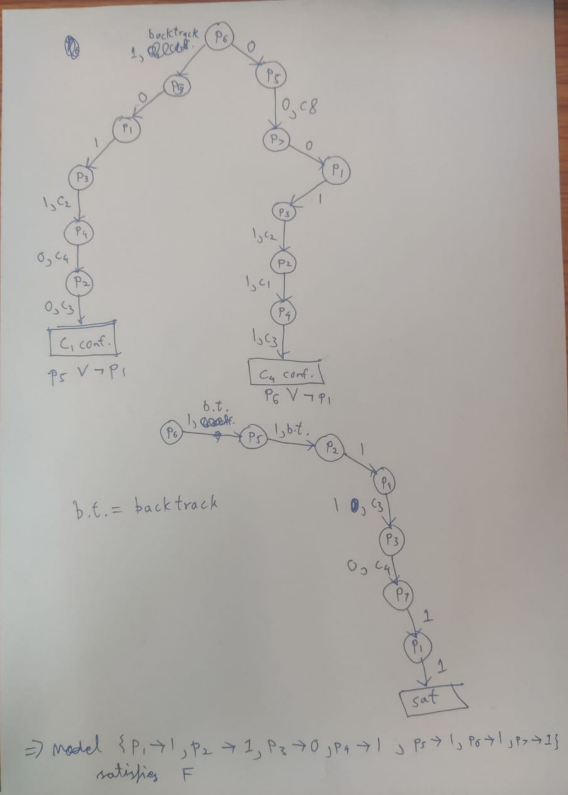
\includegraphics[scale=1]{CDCL_run.PNG}
	\caption{Exercise 11.8}
    \label{cdcl}
\end{figure}
\subsection*{Exercise 11.9}
Given any formula $F$, note that no run of the CDCL algorithm repeats a (partial) model twice, because for any partial model $m$, if $m\models F$ then the algorithm terminates, and if $m\not\models F$, then we have a conflict after performing unit propagation from $m$, following which CDCL learns a clause which thereon prevents it from repeating the model $m$. Consequently, due to the finiteness of the number of partial models on $\Vars(F)$, CDCL on $F$ must terminate.
% \section{Exercise 11.10}
% Read the first 7 pages of this \href{https://pure.tue.nl/ws/files/1766943/200207.pdf}{paper}.
\section{Tutorial 5}
Throughout this tutorial we shall use the shorthand notation $[x], x\in\mathbb{N}$ to denote the set $\{1, 2, \ldots, x\}$.
\subsection*{Exercise 12.9}
Let $p_{ij}$ denote if we have a queen on the square $(i, j)$, where $i, j\in [n]$. Then our SAT encoding is
$$\underbrace{\sum_{i = 1}^n\sum_{j = 1}^n p_{ij} = n}_{\text{We have $n$ queens}}$$
$$\bigwedge_{\text{$(i, j)$ and $(i', j')$ attack each other}} p_{ij}\Rightarrow\lnot p_{i'j'}$$
Note that $(i, j)$ and $(i', j')$ attack each other if and only if at least one of the following conditions hold:-
\begin{enumerate}
    \item $i = i'$
    \item $j = j'$
    \item $i + j = i' + j'$
    \item $i - j = i' - j'$
\end{enumerate}
\subsection*{Exercise 12.11}
Suppose we have $\ell$ sets $\{S_i\}_{i\in[\ell]}$ such that $S_i\subseteq[n]$ and $|S_i| = k$ for every $i\in [\ell]$. Further, we also have $|S_i\cap S_j| = 1$ for all distinct $i, j\in[\ell]$.\\
Consider the propositional variables $\{p_{ij}\}_{i\in [n], j\in [\ell]}$, where $p_{ij}$ is true if $i\in S_j$. Then the constraints of our problem dictate 
$$F_\ell := \underbrace{\bigwedge_{j\in [\ell]}\left(\sum_{i\in[n]}p_{ij} = k\right)}_{\text{Every set has size $k$}}\wedge\underbrace{\bigwedge_{1\leq j_1 < j_2 \leq\ell}\left(\sum_{i\in [n]}p_{ij_1}\wedge p_{ij_2} = 1\right)}_{|S_{j_1}\cap S_{j_2}| = 1}$$
Finally, to encode the maximality of our set family, we write 
$$G_\ell := F_\ell\wedge\lnot F_{\ell + 1}$$
$$F := \bigvee_{\ell = 1}^{\binom{n}{k}} G_\ell$$
Note that we implicitly assume that $\Vars(G_{\ell_1})\cap\Vars(G_{\ell_2}) = \Vars(F_{\ell_1})\cap\Vars(F_{\ell_2}) = \emptyset$ if $\ell_1\neq \ell_2$, ie:- we generate fresh variables every time we generate a different $F_\ell, G_\ell$. In particular, note that the variables of $F_\ell$ in $G_{\ell}$ and the variables of $F_\ell$ in $G_{\ell - 1}$ are distinct. \\
Now note that exactly one clause in $F$ is positive for a satisfying model of $F$, ie:- if $\ell_0$ is the \textbf{maximum}\footnote{note that we were only asked to find a maximal family. We went ahead and found a maximum one, which is also obviously maximal} size of a pairwise 1-intersecting $k$-family, then $F_{\ell_0}\wedge\lnot F_{\ell_0 + 1}$ is positive, and no other clause is.\\
Thus a satisfying assignment yields to us the maximum size of the desired family, as well as a possible family itself, which can directly be read off from the values of the propositional variables.
\subsection*{Exercise 13.7}
Refer to \autoref{z31}, \autoref{z32}.\\
Credits to Amit Rajaraman for this code.
\begin{figure}[h]
	\centering
	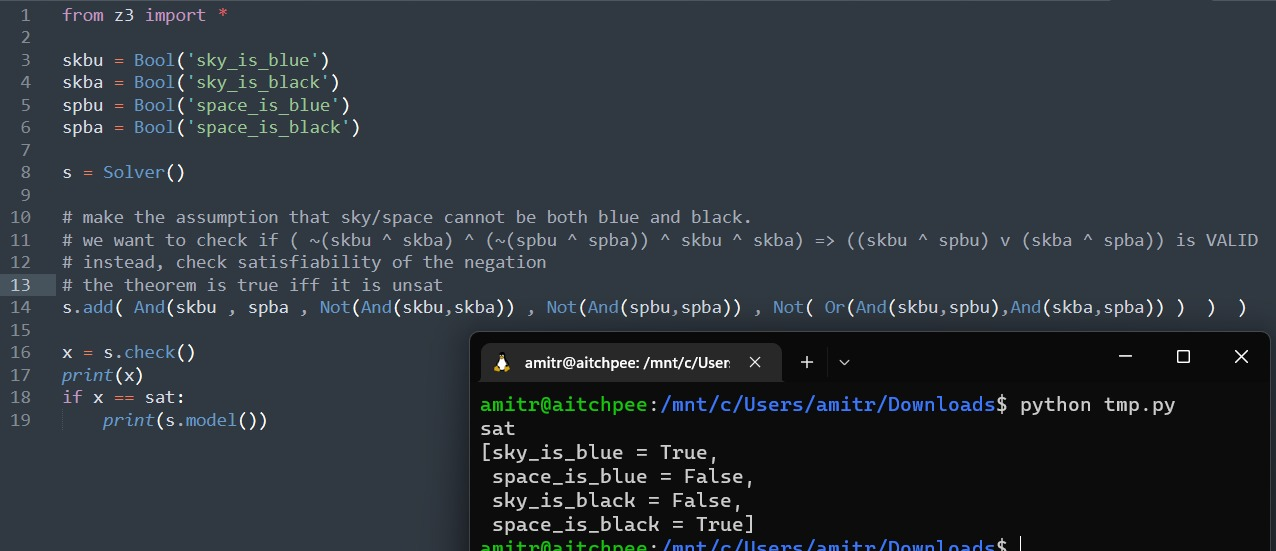
\includegraphics[scale=0.3]{z31.jpeg}
	\caption{Exercise 13.7}
    \label{z31}
\end{figure}
\begin{figure}[h]
	\centering
	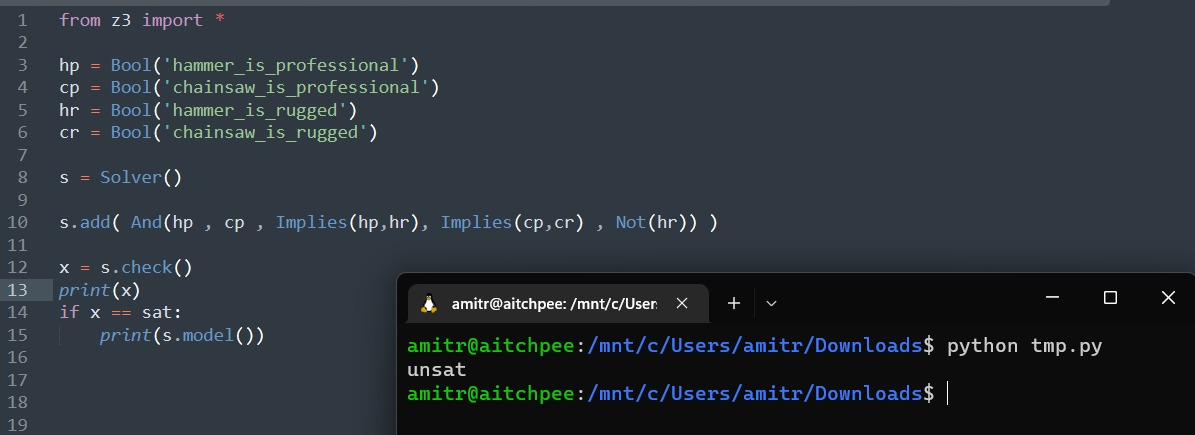
\includegraphics[scale=0.3]{z32.jpeg}
	\caption{Exercise 13.7}
    \label{z32}
\end{figure}
\subsection*{Exercise 13.8}
Draw a parse tree of the formula, and carry out a standard tree traversal of the parse tree, keeping a count of how many $\lnot$ we have encountered so far. Whenever we reach a leaf, if the number of $\lnot$ seen so far is even, then that leaf occurs positively, otherwise not. A variable $p$ occurs positively iff every leaf corresponding to $p$ occurs positively.
\end{document}